\section{Task and Setting}
\label{sec:task}
Our assignment is a small but demanding robot-packing task in the A3 dual-arm MuJoCo simulator~\cite{a3}. A robot must move thin, closely packed cookies from a \emph{source box} into a \emph{target box}. It must take the correct number of cookies in each grasp and place them neatly without leaving cookies hanging over an edge, knocking over its earlier work, or accidentally dragging extra cookies out of the source.

There are two tasks. In \pFive, the robot transfers two groups of five cookies, making ten target cookies. In \pTen, it makes four transfers: first $n$ cookies, then $10-n$, and repeats that pattern for the second target column. The first-group size $n$ may vary between trials. Thus, \pTen\ is not merely a longer \pFive: the robot must handle a thin single cookie as well as a large group, and the first group affects the space available for later ones.

The source has four columns, each containing twenty cookies. The course's standard six-setting evaluation uses \srcone; the simulator also supports selecting the other three columns. Each task is tested under \emph{Basic}, \emph{Medium}, and \emph{Advanced} scene variation. The environment changes relevant box and cookie positions, camera parameters, lighting, and, for the hardest setting, cookie colors. These changes are applied by the official benchmark, not by our policy.

\paragraph{What the robot can know.}
The policy receives RGB images from a front camera and two wrist cameras, together with public robot motion and gripper/force observations. It can use the known shape of the robot and its fingers. It does not read the simulator's hidden positions of cookies to decide what to do. During development, the evaluator records such hidden information separately, so we can explain a failure after a run without giving the policy an unfair advantage.

\paragraph{What counts as success.}
The teacher's final score uses two complementary measures. \emph{Completion} counts how many cookies end in valid target positions; \emph{success} requires the entire task to satisfy the simulator's placement and source-box conditions. For example, ten cookies may appear to have arrived in \pFive, but disturbing a separate cookie in the source can still make the run unsuccessful. This distinction shaped much of our later work.

\section{The AI Advisor--Executor Workflow}
\label{sec:workflow}
The policy was built in an iterative collaboration between a human team and AI assistants. It is useful to distinguish their roles because the project is about \emph{improving software through experiments}, not training one neural model to control the robot.

\begin{figure*}[t]
\centering
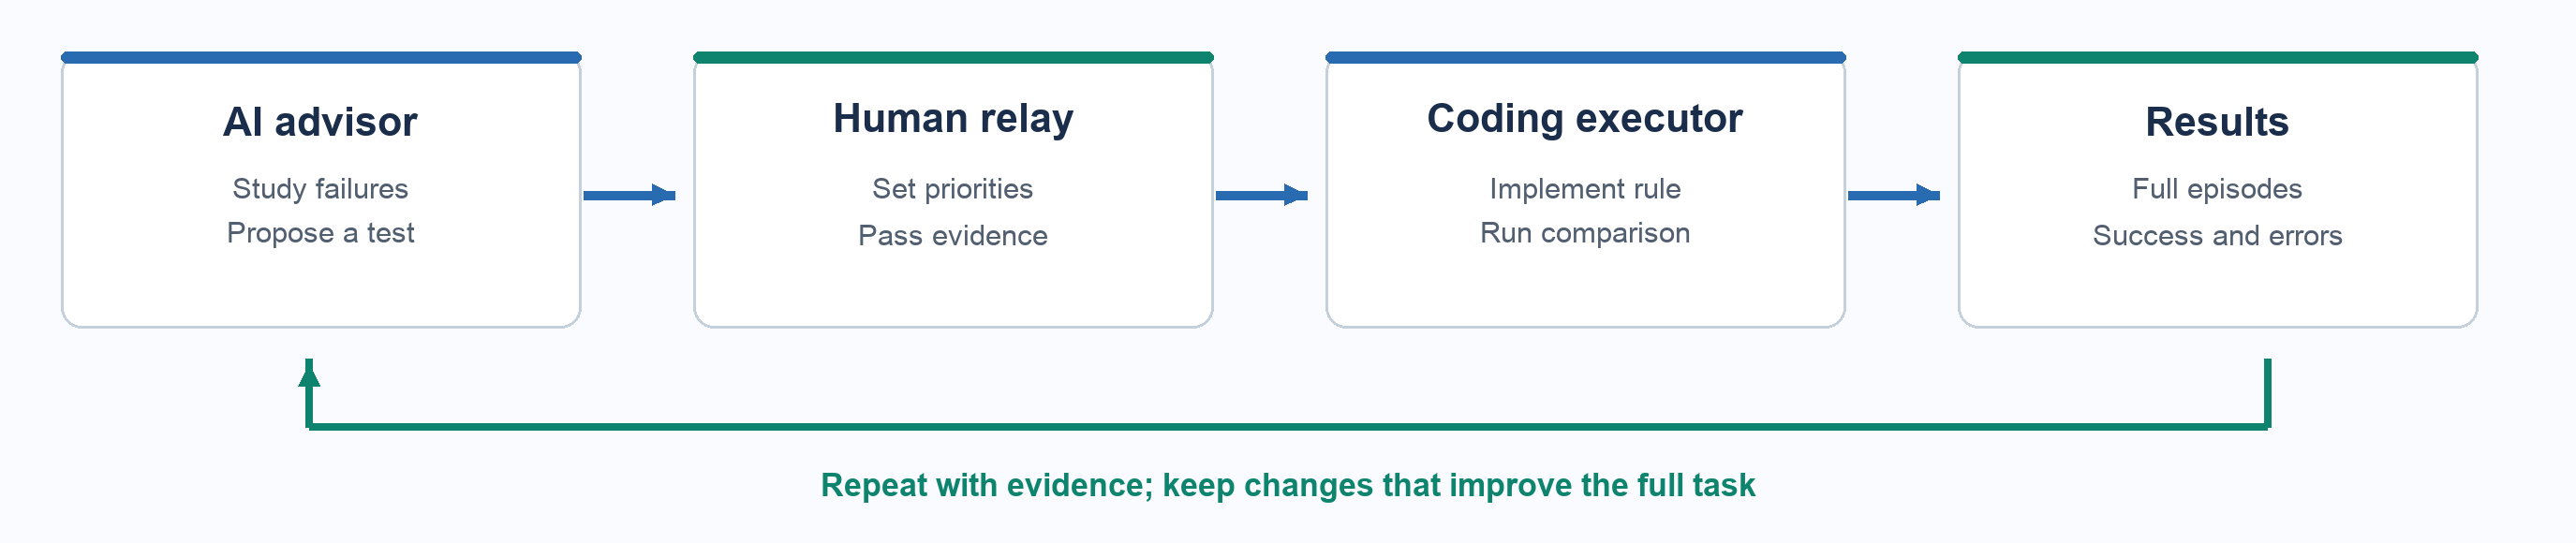
\includegraphics[width=0.99\textwidth]{figures/advisor_executor_loop.png}
\caption{The development loop. The advisor diagnoses and proposes a focused change; the human team relays the plan and sets priorities; a coding executor implements and tests it; the resulting successes and failures guide the next iteration.}
\label{fig:advisor}
\end{figure*}

\paragraph{Advisor: decide what to investigate.}
The advisor was GPT-6 in the Astra configuration. It read run summaries, inspected source code and failure evidence, compared alternative explanations, and proposed concrete experiments. Its main output was a decision such as: \emph{check whether the robot is following an outdated box position before changing the grasp force}. The advisor also decided whether promising small-test changes deserved a larger evaluation and which regressions mattered.

\paragraph{Executor: make and measure the change.}
The coding executors were separate, high-reasoning agent processes, including GPT-6.1 Sol (xhigh), GLM-5.3 (xhigh), and DeepSeek V4 Flash 1017 (high), as available at different stages. They worked on local files and the authorized compute machines. An executor typically read the preceding implementation, modified the Python policy, ran simulator trials, collected errors, and returned results and saved code. This separation let the advisor reason about the overall approach while the executor handled the detailed implementation and repeated tests.

\paragraph{Human team: coordinate and verify.}
Group 3 set the research goal, chose the rule-based approach, transferred plans and results between otherwise separate agent sessions, checked important decisions, and assembled the final submission. In practice, the human often acted as the messenger between advisor and executor. The files exchanged were plans, code locations, experimental outputs, and short summaries rather than a single uninterrupted AI conversation.

\paragraph{One iteration in practice.}
The working cycle had five steps:
\begin{enumerate}[leftmargin=1.45em,itemsep=1pt,topsep=2pt]
\item \textbf{Find the first meaningful failure.} Was a group misidentified, missed during grasp, lost while carrying, or placed incorrectly?
\item \textbf{Write a small, testable explanation.} For instance, the target camera may be seeing an old object position.
\item \textbf{Make one targeted change.} Keep unrelated parts of the controller unchanged.
\item \textbf{Test both failures and previous successes.} Compare the new code with the old version on matched seeds where possible.
\item \textbf{Keep, revise, or discard.} Freeze a version only when its complete-run results justify the change.
\end{enumerate}

This process made a useful distinction between an attractive idea and a successful policy. Some changes solved one visible problem but created another. We kept those negative results and used them to narrow later improvements. Figures~\ref{fig:advisor} and~\ref{fig:controller} illustrate the software-development loop and the robot's own feedback loop, which operate at different time scales.
